
In the proposed architecture, the \textit{SmartBox} plays the role of acquiring the data that is transmitted wirelessly by the \textit{Biostickers}, which can be seen on Figure \ref{fig:biosticker-imgs}.
Each \textit{SmartBox} is associated to a single patient, it captures the data of each \textit{Biosticker} attached to that patient, and stores it in a local database for redundancy. 
It should also be capable of analyzing and process the data in real time, before propagating it to the higher layers in the system architecture, in order to reduce computation and networking overhead on the Smart Gateway. The \acs{WoW} project also foresees the usage of a classification algorithm in the \textit{SmartBox} to determine the body pose of the patient, as well as filtering the respiration data to account for signal fluctuations caused by sudden movements by the patient.  

\begin{figure}[H]
    \begin{minipage}[r]{0.74\linewidth}
        \includegraphics[width=\linewidth]{images/biosticker imgs/test.png}
    \end{minipage}
    \begin{minipage}[l]{0.25\linewidth}
        \includegraphics[width=\linewidth]{images/biosticker imgs/a.png}
        \includegraphics[width=\linewidth]{images/biosticker imgs/b.png}
        \includegraphics[width=\linewidth]{images/biosticker imgs/c.png}
    \end{minipage}
    \centering
    \caption[Illustration of the \textit{Biostickers}.]{Illustration of the \textit{Biostickers}. On the left, a conceptual illustration of the different components that form the \textit{Biosticker} is shown. On the right, photographies of a test volunteer using the \textit{Biosticker} are exhibited.}
    \label{fig:biosticker-imgs}
\end{figure}


\paragraph{} Additionally, for debugging purposes, researchers at the \acs{ISR} developed a simple developer \acs{GUI}, which can be seen on Figure \ref{fig:smartbox-gui}.

\begin{figure}[H]
    \centering
    \includegraphics[width=\linewidth]{images/smartbox-gui.png}
    \caption{Illustration of the developer \acf{GUI} for debugging the \textit{SmartBox} acquisition, designed by the \acs{WoW} research team at \acs{ISR}.}
    \label{fig:smartbox-gui}
\end{figure}

\paragraph{} Regarding data acquisition, the \textit{SmartBox} collects 5 distinct biosignals, which can be seen on the developer low level \acs{GUI} on Figure \ref{fig:smartbox-gui}:

\begin{itemize}
    \item \acf{ECG} -- Byte array (20 byte length) with the electrical signal measured, with a frequency of 20Hz.
    \item Respiration Rate -- An unsigned integer (4 bytes) representation of the rate of respiration, with a frequency of 10Hz.
    \item Heart Rate -- An unsigned byte representation of the heart rate in \textit{beats per minute}, every 5s.
    \item Body Temperature -- An IEEE 11073\footnote{\url{https://standards.ieee.org/standard/11073-10207-2017.html}} floating-point number representation of the body temperature, every 60s.
    \item Oxygen Saturation -- A standard floating-point number (4 bytes) representation of the oxygen saturation, with a frequency of 1Hz.
\end{itemize}

\todo[inline]{Todo: Confirm with @Bernardo acquisition rates for each value.}
\todo[inline]{Todo: Ask @Miguel for a picture of the biostickers.}
\section{Deciding on a Hardware Platform}

In the context of this dissertation, two different \acl{SBC}s (\acs{SBC}) were considered for the development of the \textit{SmartBox}: a Raspberry Pi 4 Model B and an UDOO BOLT v3. In the following sections we discuss and compare the characteristics of each platform. 

\subsubsection{Raspberry Pi 4 Model B}

Raspberry Pi denotes a series of \acs{SBC}s which are developed by the Raspberry Pi Foundation, a UK-based charity that aims to educate the general public about the power of computing and digital making, in association with Broadcom. It is one of the most popular hardware platforms used by developers due to its accessible price and community support \cite{jain2021introduction}.
At the time of the writing, the Raspberry Pi 4 Model B (or Raspberry Pi 4B)\footnote{\url{https://www.raspberrypi.com/products/raspberry-pi-4-model-b/}}, which can be seen in Figure \ref{fig:raspberrypi-image}, is the latest revision of the Raspberry Pi series, powered by Broadcom BCM2711 System on a Chip (SoC).

\begin{figure}[H]
    \centering
    \includegraphics[width=\linewidth]{images/raspberry-4-modele-b-4go.jpg}
    \caption{Raspberry Pi 4B.}
    \label{fig:raspberrypi-image}
\end{figure}

\subsubsection{UDOO BOLT V3}

As stated by the manufacturer\footnote{Product Website: https://www.udoo.org/discover-the-udoo-bolt/}, the ``UDOO BOLT is a quantum leap compared to current maker boards''. It represents a series of high performance \acs{SBC}, equipped with the latest generation of AMD Ryzen Embedded SoC. Additionally, it contains an Arduino Compatible microcontroller (connected via UART), making the UDOO BOLT extremely versatile.
The UDOO Bolt is incredibly well-supported by UDOO but unfortunately, it does not have nearly the same community support of Raspberry Pi.

\paragraph{} The UDOO BOLT V3, which can be seen in Figure \ref{fig:udoobolt-image}, is the entry-level product of the series, but it is still capable of allegedly outperforming full-fledged computers such as the Apple MacBook Pro 13", which just goes to show how powerful these \acs{SBC}s can be.

\todo[inline]{To-do: If time allows it, remake this with better quality.}

\begin{figure}[H]
    \centering
    \includegraphics[width=\linewidth]{images/UDOO_BOLT_GEAR_BLT.png}
    \caption{UDOO BOLT V3.}
    \label{fig:udoobolt-image}
\end{figure}

\subsection{Comparing the Hardware Platforms}

In order to decide on which platform to pick for the development of the project, it is crucial to compare the specification of both boards, which can be seen in the Table \ref{tab:comparsion-hardwareplatform}.

\paragraph{} From Table \ref{tab:comparsion-hardwareplatform}, we immediately conclude that the Raspberry Pi is a much more affordable alternative. At over 1/7 of the price, it already has a working WiFi+BT networking module (which is not included in the UDOO BOLT), nearly identical Input/Output (I/O) port capability and a smaller size. UDOO BOLT V3 on the other hand, has a much better SoC, which is expected to delivery a much better overall computing performance.

\renewcommand{\arraystretch}{2.5}
\begin{table}[H]
    \centering
    \begin{tabular}{r|l|l}
        %\textbf{Features} 
        & \textbf{Raspberry Pi 4B}& \textbf{UDOO BOLT V3}  \\ \hline
        \textbf{SoC} &  \makecell{Broadcom BCM2711 \\ (ARMv8 64-bit) \\ 4-core @ 1.5GHz} & \makecell{AMD Ryzen™ Embedded V1202B \\ (AMD64 64-bit) 2-core @ 2.3GHz \\ (up to 3.2GHz turbo)}\\
        \textbf{RAM} & 2, 4 or 8GB LPDDR4 & Up to 32GB DDR4 (Not included) \\ 
        \textbf{Storage} & \makecell{No internal storage, \\ SDXC Card Support} & \makecell{32GB internal eMMC + \\1 × SATA III and \\ 2 × M.2 connectors}\\
        \textbf{Networking} & \makecell{2.4/5.0 GHz WiFi, Gigabit \\ Ethernet, Bluetooth 5.0, BLE} & \makecell{Gigabit Ethernet + M.2 Key E slot \\ for optional WiFi+BT module}\\ 
        \textbf{I/O Ports} & \makecell{ 2 × USB 3.0, 2 × USB 2.0, \\ 2 × (Mini) HDMI} & \makecell{2 × USB 3.0 Type-A, \\ 2 × USB Type-C (w/ Display Port \\ + Power Delivery), 2 × HDMI} \\
        \makecell[r]{\textbf{Other} \\\textbf{Features}} & \makecell{Power over Ethernet \\(PoE)–enabled} & \makecell{Includes ATmega32U4 microcontroller\\ (Arduino Leonardo compatible), \\ RTC Battery} \\   
        \textbf{Dimensions} & 8.5 x 5.6 x 1.7 cm & 12 x 12 x 7 cm \\
        \textbf{Price} & \makecell{75.93 € (\textbf{8GB Model}, \\ including a 32GB SDXC Card\\ and case)} & \makecell{534.48 € (including external power \\ supply and a 16GB RAM module)} \\
    \end{tabular}
    \caption{Specifications of the Raspberry Pi 4B and UDOO BOLT V3.}
    \label{tab:comparsion-hardwareplatform}
\end{table}
\renewcommand{\arraystretch}{1}

\paragraph{} In order to understand how these differences in the hardware specification between the \acs{SBC}s translate to real-world performance, a test suite was developed and conducted to quantify the performance of each \acs{SBC}. The tools developed for each test can be found here\footnote{\url{https://github.com/WoW-Institute-of-Systems-and-Robotics/smartbox\_benchmark\_tests}}. 

\paragraph{}Below, we detail how each test works and discuss how each \acs{SBC} performed. 

\subsubsection{Test 1: Python Benchmark}

Given the data processing requirements for the \textit{SmartBox}, and as Python will be used as the main scripting language for most of the \textit{SmartBox} development, we developed a simple test to estimate computing performance, or more specifically (single-threaded) performance of arithmetic tasks, on each \acs{SBC}. In this test, each \acs{SBC} calculates the \textit{n}-th number in the Fibonacci sequence \cite{pierce1951fibonacci}, and we measure the time taken. This process is repeated 10 times for different numbers, from 10000 to 500000, to determine average run time.

\begin{figure}[H]
    \centering
    \includegraphics[width=0.8 \linewidth]{images/fibonacci-test.pdf}
    \caption [Custom Python benchmark for the Raspberry Pi 4B and UDOO BOLT V3.]{ Custom Python benchmark for the Raspberry Pi 4B and UDOO BOLT V3. The standard deviation for each run time is inferior to 0.1\% in each test, and therefore it is not displayed in the figure.}
    \label{fig:fibonacci-tests}
\end{figure}

From Figure \ref{fig:fibonacci-tests}, we can observe that the time taken for computing each number increases exponentially for each platform. By analyzing the data, we can see that the UDOO BOLT V3 outperforms Raspberry Pi 4B on average by a factor of 2.5 $\pm$ 0.2.

\subsubsection{Test 2: Phoronix Test Suite}

The Phoronix Test Suite\footnote{Phoronix Test Suite - Linux Testing \& Benchmarking Platform, Automated Testing, Open-Source Benchmarking: \url{https://www.phoronix-test-suite.com/}} is an open-source benchmarking platform used for comparing the performance of different systems. The framework provides compilations of tests for a variety of tools and is also fully customizable and expandable, allowing users to develop and automate their own tests in a clean, reproducible and easy-to-use fashion. The test profiles work by measuring some property of the benchmark, (\textit{e.g.} the run time for calculating the first 100 Fibonacci numbers) and use it to provide an estimate of the performance of the \acs{SBC}, which can be easily used for comparison between different systems. 

\paragraph{} For the purposes of evaluating the computing performance of each \acs{SBC}, we chose the following standard test profiles provided by Phoronix\footnote{OpenBenchmarking.org - Cross-Platform, Open-Source Automated Benchmarking Platform: \url{https://openbenchmarking.org/}}, which are a compilation of the most popular Python and CPU benchmarks used \footnote{The benchmark results obtained were published in the \textit{OpenBenchmarking.org} website, and can be found by visiting the following webpage: \url{https://openbenchmarking.org/result/2110255-JNCF-211025851}.}:

\begin{itemize}
    \item BYTE Unix Benchmark (``BYTE''), single-threaded CPU benchmark -- Runs BYTE UNIX benchmark suite (more particularly, the Dhrystone 2 synthetic benchmark) to measure the amount of instructions per second (IPS). 
    \item 7-Zip Compression (``7-Zip''), multithreaded CPU benchmark -- Runs the benchmark feature integrated in 7-Zip to measure the amount of millions instructions per second (MIPS). The benchmark consists of a LZMA data compression and decompression test run, using all available threads in the system (meaning it will scale highly with the amount of threads in the system). 
    \item PyBench Benchmark (``PyBench''), single-threaded Python \& CPU benchmark -- Executes different function such as built-in function calls and nested for-loops and measures its runtime.
    \item PyPerformance \textit{chaos} Benchmark (``chaos''), single-threaded Python \& CPU benchmark -- Create chaos game-like fractals \cite{Jeffrey1992} and measures its run-time. 
    \item PyPerformance \textit{float} Benchmark (``float''), single-threaded Python \& CPU benchmark -- Create 100,000 random floating-point numbers and calculate the co-sine, sine and square root of each one and measures its run-time.
    \item PyPerformance \textit{nbody} Benchmark (``nbody''), single-threaded Python \& CPU benchmark -- Runs an \textit{n-body} problem simulation \cite{Playne2009} and measures its run-time.
    \item PyPerformance \textit{json\_loads} Benchmark (``json''), single-threaded Python \& CPU benchmark -- Evaluates \acf{JSON}\footnote{The JavaScript Object Notation (JSON) Data Interchange Format: \url{https://www.rfc-editor.org/rfc/rfc8259.html}} parsing and serialization, a widely used open stardard data format, by dumping and loading thousands of objects and measures its runtime.
    \item PyPerformance \textit{crypto\_pyaes} Benchmark (``crypto''), single-threaded Python \& CPU benchmark -- Runs the AES block-cipher Python implementation and measures its run-time.
    \item PyPerformance \textit{regex\_compile} Benchmark (``regex''), single-threaded Python \& CPU benchmark -- Compiles different \textit{regular expressions} or \textit{regexes} in Python and measures its run-time.
    \item PyPerformance \textit{python\_startup} Benchmark (``startup''), single-threaded Python \& general system performance benchmark -- Measures Python's startup time.
    \item PyPerformance \textit{django\_template} Benchmark (``django''), single-threaded Python benchmark -- Builds a 150x150-cell HTML table and measures its run-time.
\end{itemize}

\begin{figure}[H]
    \centering
    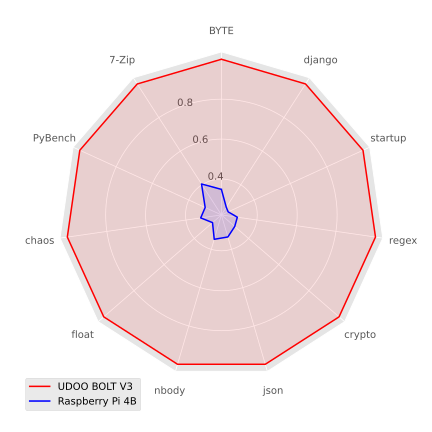
\includegraphics[width=0.8 \linewidth]{images/phoronix-benchmarks.pdf}
    \caption [Phoronix benchmarks for the UDOO BOLT V3 and Raspberry Pi 4B.]{ Phoronix benchmarks for the UDOO BOLT V3 and Raspberry Pi 4B. The performance values for each test are normalized to UDOO BOLT V3 performance.}
    \label{fig:phronix-benchmarks}
\end{figure}

\paragraph{} From Figure \ref{fig:phronix-benchmarks}, we can observe that UDOO BOLT V3 performs much better than Raspberry Pi 4B in every benchmark, as expected. We also notice some disparity in the relative performance throughout the benchmarks, in particular, the 7-Zip benchmark. This is likely due to the fact that 7-Zip benchmark is a multithreaded test, and as Raspberry Pi 4B has more threads than UDOO BOLT V3, it manages to close the performance gap (albeit only slightly). By analyzing the data, we find that UDOO BOLT V3 outperforms Raspberry Pi 4B on average by a factor of 2.21 $\pm$ 0.4.

\subsubsection{Test 3: \acs{MQTT} Benchmark}

As the \textit{SmartBox} is intended to communicate with the \textit{Smart Gateway} through \acs{MQTT} messages, we also evaluate how each system handles the load associated with an \acs{MQTT} client. For this test, each \acs{SBC} ran a simple \acs{MQTT} client, which subscribes to a single topic and publishes a message to another topic at a given transmission rate, with a payload containing the string ``hello world'', through an \acs{MQTT} broker in the local network.

\todo[inline]{To-do: Repeat tests with higher rates if time allows it.}
\begin{figure}[H]
    \centering
    \includegraphics[width=\linewidth]{images/mqtt_test_results.pdf}
    \caption[\acs{MQTT} benchmark for Raspberry Pi 4B and UDOO BOLT V3.]{\acs{MQTT} benchmark for Raspberry Pi 4B and UDOO BOLT V3. As the transmission frequency increases, we observe that the Raspberry Pi consumes more resources than the UDOO BOLT V3, nonetheless, these are very negligible performance differences, with an impact of < 0.5\% resource usage.}
    \label{fig:mqtt-tests}
\end{figure}

The \acs{MQTT} client is a very lightweight process, and as seen in Figure \ref{fig:mqtt-tests}, it is capable of running on both platforms with trivial performance impact.

\subsection{Final Decision on SmartBox hardware}

Based on the results of our tests we conclude that UDOO BOLT V3 heavily outperforms the Raspberry Pi 4B in CPU benchmarks, but shows a negligible difference in memory usage. Nonetheless, we find that these performance gains do not meaningfully impact the \textit{SmartBox} functionality, for example, in the \acs{MQTT} communication. We can also extend this to other features, such as the developer \acs{GUI} or the Python acquisition script, which should have a similar resource load to the \acs{MQTT} client in the previous \acs{MQTT} benchmark.

\paragraph{} Additionally, the Raspberry Pi 4B comes out of the box with an included WiFi+\acs{BLE} combo networking card, 8GB of RAM (as we chose the 8GB model), and a much smaller form factor -- which is very useful for embedding the \textit{SmartBox} in the \textit{SmartBeds}. And this is at 1/7 the cost of UDOO BOLT V3, making this much more affordable to scale and replicate the system with many \textit{SmartBoxes}.

\paragraph{} Due to all of the aforementioned reasons, we have decided to move forward with the Raspberry Pi 4B for the \textit{SmartBox} development in the scope of the \acs{WoW} project.

\section{Communication with the Biostickers}

As previously mentioned, the communication between the \textit{Biostickers} and the \textit{SmartBox} makes use of the \acs{BLE} protocol. One of the advantages of using the Raspberry Pi 4B, as discussed in the previous section, is the fact that it already includes all networking functionality needed for the project. 

% explicar pra que serve e q sinal adquire

\paragraph{} However, the communication with the \textit{Biostickers} is very critical and demanding. During the development of the project, the research team has decided to use a \textit{Biosticker} coupled with a commercially available Pulse Oximeter -- used to measure oxygen saturation at the finger tip --  in order to capture all required biosignals. This means that the \acs{BLE} acquisition system must be capable of handling both communications simultaneously. Having this in mind, we need to understand if the included \acs{BLE} adapter of the Raspberry Pi board is sufficient for the task, or if we need to consider a different acquisition hardware.

\paragraph{} In order to understand how data transmission works between \acs{BLE} devices, some technical background regarding the data transmission in protocol is presented.

\subsection{Technical Background} 
 % Ver https://www.scirp.org/journal/paperinformation.aspx?paperid=103686

% \todo[inline]{To-do: Intro to Link Layer, LE 1M e 2M, packet format, mention GATT and overview data transmission...}

\paragraph{} Before we discuss \acs{BLE} data transmissions, it is important to introduce to certain terminology which is commonly used:

\begin{itemize}
    \item Central device (or master): Device that initiates commands and requests.
    \item Peripheral device (or slave): Device that receives commands and requests, and returns responses.
    \item Connection Event: Moment of the connection where the devices engage in radio transmissions.
\end{itemize}

The \acs{BLE} protocol stack is organized into three major components, as shown in Figure \ref{fig:ble-protocol-stack}: the Application Layer, the Host Layer and Controller Layer. 

\begin{figure}[H]
    \centering
    \includegraphics[width=0.6\linewidth]{images/ble protocol stack.pdf}
    \caption[Diagram of the different components of the \acs{BLE} protocol stack.]{Diagram of the different components of the \acs{BLE} protocol stack. Adapted from \cite{Specification1999, Farej2020}}
    \label{fig:ble-protocol-stack}
\end{figure}

At the Controller layer, we have the \acf{PHY} and \acf{LL} components. 

The \acf{PHY} is the bottom layer of the \acs{BLE} stack, and is responsible for the transmission and reception of information over radio waves on the Industrial Scientific Medical (ISM) 2.4GHz band. According to the latest revision of the specification \cite{Specification1999}, \acs{BLE} supports 3 distinct physical layers: LE 1M, LE 2M and LE Coded. The first is the default \acs{PHY}, with a data rate of 1 Mbps, which existed in previous versions of Bluetooth, the latter 2 were introduced in Bluetooth 5. LE 2M is an upgrade of the previous \acs{PHY}, doubling the data rate to 2 Mbps, and LE Coded has a much larger range (up to 4x), at cost of a lower data rate (500 kbps or 125 kbps). 

The \acf{LL} layer interfaces directly with the \acs{PHY}, and manages the link state of the radio. It also provides the mechanism for the higher layers to interact with the radio transceiver. 

\paragraph{} Afterwards, we have the Host Layer, containing the higher level components of the protocol stack that interact with the application level layers. The \acs{L2CAP} is responsible for managing the data between the \acs{LL} and the higher layers in the protocol stack. It abstracts the communication details from the higher layers, handling seamlessly the fragmentation of the data into multiple \acs{LL} data packets for transmission and reassembly of \acs{LL} data packets for higher layer protocols such as \acf{ATT}.

\acs{ATT} is the protocol used to expose the application data to other \acs{BLE} devices through data structured called ``attributes'', which are smallest addressable units of data used by \acs{ATT}. These are composed of 3 properties: 

\begin{itemize}
    \item an attribute type, defined by a \acf{UUID}\footnote{\url{https://tools.ietf.org/html/rfc4122}}, which indicates the type of data that is stored in the attribute.
    \item an attribute handle, to uniquely identify that attribute on the device (which in this case has the role of a server), allowing other devices (which are clients) reference the attribute for read and write requests;
    \item a set of permissions that are defined which is defined in the \acf{GATT} layer.
\end{itemize}

However, from the application point of view, data is exchanged using \acf{GATT}. \acs{GATT} defines a service framework using the \acs{ATT} protocol, defining the procedures used to exchange data between the \acs{BLE} devices. Regarding \acs{GATT}, there are 3 main constructs to consider:

\begin{itemize}
    \item \acs{GATT} Characteristic -- The lowest level concept in \acs{GATT} transactions is the Characteristic, which encapsulates a single data point, \textit{e.g.} a temperature measurement, a accelerometer reading, etc. It also defines the different types of interactions, such as reading, writing, subscribing for notifications, etc.
    \item \acs{GATT} Service -- A collection of \acs{GATT} characteristics.
    \item \acs{GATT} Profile -- A collection of Services, usually predefined by Bluetooth SIG in order to promote interoperability, but can also be customized for the application's needs.
\end{itemize}

The \acf{SMP} handles the security in the data transmissions, containing the security algorithms used to encrypt and decrypt the communication.

\paragraph{} The Application Layer contains the user application, which interfaces with the Bluetooth protocol stack.


\paragraph{} After this overview of the different layers that compose \acs{BLE}, we are ready to engage in the analysis of the \acs{BLE} data transmission.

\subsubsection{\acs{BLE} data transmission}

\paragraph{} As seen previously, there are multiple layers that involved in the transmission of data in \acs{BLE}. Figure \ref{fig:ble-ll-packet-format} displays the format of a \acs{BLE} data packet, showing how the data is encapsulated for the transmission.

\begin{figure}[H]
    \centering
    \includegraphics[width=\linewidth]{images/bluetooth data packet format.pdf}
    \caption[Diagram of the \acs{BLE} data packet format for LE 1M \acs{PHY}.]{\acs{BLE} data packet format for LE 1M \acs{PHY}. Adapted from \cite{Specification1999, Farej2020}. The Message Integrity Check (MIC) and Cyclic Redundancy Check (CRC), which are not discussed above, are used for validating the integrity of the data packet.}
    \label{fig:ble-ll-packet-format}
\end{figure}

\paragraph{} Communication in \acs{BLE} works in a particular manner, instead of having the devices transmit data whenever there is new information to exchange, the devices concentrate their radio transmissions in a brief time frame that occurs periodically called the Connection Event. This allows devices to heavily reduce power consumption, as they can negotiate the amount of radio ``downtime'' to minimize the amount of transmissions.

\paragraph{}  Figure \ref{fig:ble-message-sequence-chart} illustrates a single Connection Event during a \acs{BLE} communication between two devices, A and B. When the device A wants to communicate to the device B, the data must be first fragmented into different \acs{LL} data packets on the \acs{L2CAP} layer, which for this simple example is not considered. The data is transmitted to device B through the \acs{LL} layer, and the data is then reassembled on device B. 

\paragraph{} One thing to consider is that, although there are not rules restricting the amount of data packets that are exchanged during a Connection Event, some \acs{BLE} protocol stack implementations may not support sending more than one packet per Connection Event.


\begin{figure}[H]
    \centering
    \includegraphics[width=\linewidth]{images/ble-sending-data.pdf}
    \caption[Message sequence chart between two \acs{BLE} devices during a Connection Event.]{Message sequence chart between two \acs{BLE} devices during a Connection Event. Adapted from \cite{Specification1999}}
    \label{fig:ble-message-sequence-chart}
\end{figure}

\paragraph{} There are multiple parameters which guide how \acs{BLE} data connections are performed, which are the following: 
\begin{itemize}
    \item Slave Latency: Number of consecutive connection events the slave device is not required to listen for the master. It allows a slave to use a reduced number of connection events, thus minimizing power consumption.
    \item Connection Interval: Time between two consecutive connection events.
    \item Supervisor Timeout: Maximum time between two received data \acs{PDU}s before the connection is considered lost.
    \item \acf{MTU} for the \acs{ATT} protocol: Length of the \acs{PDU} for the \acs{ATT} protocol, which includes the \acs{ATT} header as well as the payload containing the data to be transmitted.
\end{itemize}

\subsubsection{\acs{BLE} protocol stack on Linux} 

In the \acs{WoW} project, the data acquisition is developed using the official Linux implementation of \acs{BLE} protocol stack\footnote{\textit{BlueZ}: \url{http://www.bluez.org/profiles/}} -- \textit{BlueZ} -- in order to promote interoperability; since these drivers are developed and used by the community, allowing us to use multiple \acs{BLE} adapters, and even different \acs{SBC}s, using the same codebase without being tied down to proprietary code. 

% \paragraph{} Currently, \textit{BlueZ} only officially supports up to the Bluetooth 4.2 specification, which is, at the time of writing, is still the predominantly used version \cite{Faria2020}. Nonetheless, Bluetooth specifications are generally backwards compatible with older versions.

% \todo[inline]{Nota para @David Portugal: Isto é o que está indicado no website, mas existem funcionalidades de Bluetooth 5.X que estão implementadas (mas não especificam o escopo que está implementado). Indico alguma coisa sobre isso? Removo este parágrafo? Ou deixo tudo como está? }


\subsection{Choosing a \acs{BLE} adapter} 

\paragraph{} As mentioned previously, one of the objectives of this dissertation work is to analyze if the internal \acs{BLE} adapter provided by the Raspberry Pi 4B is sufficient for the \acs{WoW} project. To achieve this, we decided to compare this adapter with a commercially available that met the requirements for the project. The requirements for the adapter are the following:

\begin{itemize}
    \item The adapter must support, at least, the Bluetooth 5.0 core specification.
    \item The adapter must natively support Ubuntu 20.04, as well as the \textit{BlueZ} \acs{BLE} protocol stack. 
    %\item The adapter should support the LE 2M physical layer for better throughput.
\end{itemize}

\paragraph{} After researching the available market, we chose the ASUS USB-BT500 USB adapter\footnote{ASUS USB-BT500 Bluetooth 5.0 USB Adapter: \url{https://www.asus.com/Networking-IoT-Servers/Adapters/All-series/USB-BT500/}} due to its affordability and availability, making it an adequate fit for the project's needs.

\paragraph{} In the next section, we perform multiple tests to evaluate the performance of ASUS USB-BT500 and the internal \acs{BLE} adapter in the Raspberry Pi 4B.

\subsection{Testing \acs{BLE} Communication} 

To ensure an \acs{BLE} adapter is capable of handling the communication on the \textit{SmartBox} side for the \acs{WoW} project, we created two different tests to evaluate their performance at different distances: a test to evaluate the roundtrip time for a single message (for different sizes), and a test to evaluate the maximum bandwidth achieveable at a given distance.

\paragraph{} For these tests, we need to ensure the conditions are very similar to those when acquiring data from the \textit{Biostickers}. To this end, we use the same microcontroller -- nRF52832 \acs{SoC} -- which is used in the \textit{Biostickers}, with our own custom firmware for the tests. Therefore, the device which is used for the tests is the nRF52-DK developer kit\footnote{\url{https://www.nordicsemi.com/Products/Development-hardware/nrf52-dk}}. The firmware for the microcontroller is built using the latest version of MbedOS\footnote{\url{https://os.mbed.com/mbed-os/}} and can be found here\footnote{\url{https://github.com/WoW-Institute-of-Systems-and-Robotics/ble-test-firmwares/}}.

\subsubsection{Test Conditions}

In order to ensure replicability and reliability of the test results, we use the same connection parameters for all tests, which are the following:

\begin{table}[H]
    \centering
    \begin{tabular}{|l|l|}
    \hline
    \textbf{Connection Interval} & 7.5ms \\ \hline
    \textbf{Slave Latency}       & 0     \\ \hline
    \textbf{Supervisor Timeout}  & 500ms \\ \hline
    \textbf{\acs{ATT} \acs{MTU} Length}      & 23 bytes   \\ \hline
    \end{tabular}
    \caption{\acs{BLE} connection parameters used for the ASUS USB-BT500 adapter.}
    \label{tab:ble-connection-values-hci1}
\end{table}

\begin{table}[H]
    \centering
    \begin{tabular}{|l|l|}
    \hline
    \textbf{Connection Interval} & 7.5ms \\ \hline
    \textbf{Slave Latency}       & 0     \\ \hline
    \textbf{Supervisor Timeout}  & 500ms \\ \hline
    \textbf{\acs{ATT} \acs{MTU} Length}      & 251 bytes   \\ \hline
    \end{tabular}
    \caption{\acs{BLE} connection parameters used for internal Raspberry Pi 4B adapter.}
    \label{tab:ble-connection-values-hci0}
\end{table}

Additionally, these tests were conducted indoors, with the devices (the \acs{BLE} adapter and the microcontroller) in clear view of each other.

\subsubsection{Test 1: Roundtrip Time Measurement}

In this first test, we measure the roundtrip time of a single \acs{ATT} data packet on a \acs{BLE} connection for different payload sizes. For this test, the nRF52-DK board exposes a custom \acs{GATT} service containing 2 characteristics: one is updated by the \textit{SmartBox} (characteristic ``A''), and one to which the \textit{SmartBox} subscribes for notifacations (characteristic ``B''). When the \textit{SmartBox} writes on characteristic ``A'', the nRF52-DK challenges the value of the characteristic ``B'', triggering the transmission of a notification to the \textit{SmartBox}. Thus, the roundtrip time measured is then the time taken to recieve the notification on characteristic ``B'' after updating the value of characteristic ``A''. The next figures display the roundtrip time graphs for different payload sizes obtained for each adapter at different distances\footnote{The error in the distance measurement was estimated using the size of the Raspberry Pi 4B and the nRF52-DK developer board in order to provide a maximum possible error for the distance.}. Each test was run 5 times to ensure the results are consistent.

\begin{figure}[H]
    \centering
    \includegraphics[width=0.75\linewidth]{images/ble-roundtrip-hci1-0cm.pdf}
    \caption[Average \acs{BLE} connection roundtrip time obtained using Raspberry Pi 4B's internal \acs{BLE} adapter at a distance of 0m.]{Average \acs{BLE} connection roundtrip time obtained using Raspberry Pi 4B's internal \acs{BLE} adapter at a distance of $0\text{m} \pm 0.2$.}
    \label{fig:ble-roundtrip-hci1-0m}
\end{figure}

\begin{figure}[H]
    \centering
    \includegraphics[width=0.75\linewidth]{images/ble-roundtrip-hci1-300cm.pdf}
    \caption[Average \acs{BLE} connection roundtrip time obtained using Raspberry Pi 4B's internal \acs{BLE} adapter at a distance of 3m.]{Average \acs{BLE} connection roundtrip time obtained using Raspberry Pi 4B's internal \acs{BLE} adapter at a distance of $3\text{m} \pm 0.2$.}
    \label{fig:ble-roundtrip-hci1-3m}
\end{figure}

\begin{figure}[H]
    \centering
    \includegraphics[width=0.75\linewidth]{images/ble-roundtrip-hci1-600cm.pdf}
    \caption[Average \acs{BLE} connection roundtrip time obtained using Raspberry Pi 4B's internal \acs{BLE} adapter at a distance of 6m.]{Average \acs{BLE} connection roundtrip time obtained using Raspberry Pi 4B's internal \acs{BLE} adapter at a distance of $6\text{m} \pm 0.2$.}
    \label{fig:ble-roundtrip-hci1-6m}
\end{figure}

\begin{figure}[H]
    \centering
    \includegraphics[width=0.75\linewidth]{images/ble-roundtrip-hci1-900cm.pdf}
    \caption[Average \acs{BLE} connection roundtrip time obtained using Raspberry Pi 4B's internal \acs{BLE} adapter at a distance of 9m.]{Average \acs{BLE} connection roundtrip time obtained using Raspberry Pi 4B's internal \acs{BLE} adapter at a distance of $9\text{m} \pm 0.2$.}
    \label{fig:ble-roundtrip-hci1-9m}
\end{figure}

\begin{figure}[H]
    \centering
    \includegraphics[width=0.75\linewidth]{images/ble-roundtrip-hci0-0cm.pdf}
    \caption[Average \acs{BLE} connection roundtrip time obtained using the ASUS USB-BT500 adapter at a distance of 0m.]{Average \acs{BLE} connection roundtrip time obtained using the ASUS USB-BT500 adapter at a distance of $0\text{m} \pm 0.2$.}
    \label{fig:ble-roundtrip-hci0-0m}
\end{figure}

\begin{figure}[H]
    \centering
    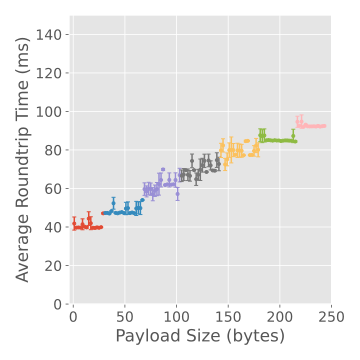
\includegraphics[width=0.75\linewidth]{images/ble-roundtrip-hci0-300cm.pdf}
    \caption[Average \acs{BLE} connection roundtrip time obtained using the ASUS USB-BT500 adapter at a distance of 3m.]{Average \acs{BLE} connection roundtrip time obtained using the ASUS USB-BT500 adapter at a distance of $3\text{m} \pm 0.2$.}
    \label{fig:ble-roundtrip-hci0-3m}
\end{figure}

\begin{figure}[H]
    \centering
    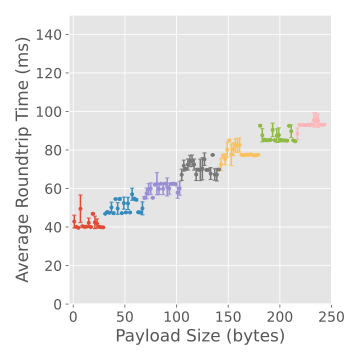
\includegraphics[width=0.75\linewidth]{images/ble-roundtrip-hci0-600cm.pdf}
    \caption[Average \acs{BLE} connection roundtrip time obtained using the ASUS USB-BT500 adapter at a distance of 6m.]{Average \acs{BLE} connection roundtrip time obtained using the ASUS USB-BT500 adapter at a distance of $6\text{m} \pm 0.2$.}
    \label{fig:ble-roundtrip-hci0-6m}
\end{figure}

\begin{figure}[H]
    \centering
    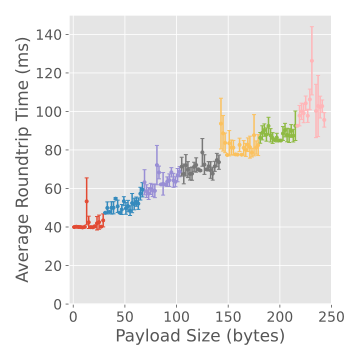
\includegraphics[width=0.75\linewidth]{images/ble-roundtrip-hci0-900cm.pdf}
    \caption[Average \acs{BLE} connection roundtrip time obtained using the ASUS USB-BT500 adapter at a distance of 9m.]{Average \acs{BLE} connection roundtrip time obtained using the ASUS USB-BT500 adapter at a distance of $9\text{m} \pm 0.2$.}
    \label{fig:ble-roundtrip-hci0-9m}
\end{figure}

\paragraph{} During the development of these tests, we discovered an functionaly which was not documented in the specification -- \acf{DLE}. This feature, introduced in Bluetooth 4.2, allows \acs{LL} data packet payload to increase significantly in size, up to 251 bytes (compared to the 23 bytes when not using this feature). This gives a head start for the ASUS USB-BT500, as it is capable of sending over 10 times more data in a single packet, compared to the Raspberry Pi 4B's internal \acs{BLE} adapter. Raspberry Pi 4B's internal \acs{BLE} adapter can handle a maximum of 20 bytes and ASUS USB-BT500 can handle up to 244 bytes (in the \acs{ATT} payload).

\paragraph{} Nonetheless, we find that for both adapters, the minimum roundtrip time is the same: appoximately 40ms. This is an odd value, given that the connection interval was set to 7.5ms, meaning the time it takes to transmit a single message and recieve it on the \textit{SmartBox} takes more than 4 connection intervals, which is nearly double of what should be expected (one interval for the transmission of the packet to the nRF52-DK and one interval to retrieve the packet). Since the roundtrip time accounts for both the transmission and reception of the data packet, this means we likely dealing with a $\sim$12ms delay in every transmission / reception.

\paragraph{} We also notice that the graphs for the ASUS USB-BT500 tests, in particular on Figure \ref{fig:ble-roundtrip-hci0-0m}, that the roundtrip graphs have a shape similar to that of a ``stepping function''. By analyzing the data from Figure \ref{fig:ble-roundtrip-hci0-0m}, we find that on average each step has a width of $34.6 \pm 3.5$ bytes, and a height difference of $8.95 \pm 1.22$ms (which is quite close to the connection interval, 7.5ms).

\paragraph{} This likely indicates that the data is being fragmented on the \acs{L2CAP} every $\sim$34 bytes (which should be the maximum size for a single connection event), and split across multiple connection intervals, instead of being transmitted in a single packet. 

Additionally, this indicates that the observed delay is most likely a bottleneck on the \textit{BlueZ} Linux \textit{API}, delaying the transmission of data from the user level to the lower levels of the \acs{BLE} protocol stack, as the roundtrip time increases in increments of the connection interval with the payload size, pointing to an issue on the \acs{BLE} stack implementation instead.

Also, this indicates that to maximize data throughput, we should use the maximum supported payload size, in order to minimize the impact of the the initial $\sim$12ms delay on the transmission.
 
\paragraph{} We can also observe that for both adapters, the roundtrip times measurements become significantively noisy as the distance increases, as expected, although it is particularly noticable for the Raspberry Pi 4B's internal \acs{BLE} adapter on Figure \ref{fig:ble-roundtrip-hci1-9m}. 

\paragraph{} 

\subsubsection{Test 2: Bandwidth Measurement}

In this second test, we measure the maximum bandwidth for the \acs{BLE} connection by adjusting the transmission rate, or more accurately, the time between the transmission of each packet. 

For this test, the nRF52-DK board exposes 7 \acs{GATT} characteristics\footnote{This behaviour is not documented on the \textit{BlueZ} documentation, but it was empirically determined by the author to be the maximum number of concurrent characteristics which can be used before the connection crashes, for both adapters.} for the \textit{SmartBox} to subscribe to. The nRF52-DK then continuously changes the value of the characteristic, immediately triggering a notification to the \textit{SmartBox} -- one for each characteristic. The transmission rate was increased until the connection became too unstable and crashed. The payload size used on each characteristic corresponds to the maximum payload detected in the roundtrip test -- 20 bytes for the internal \acs{BLE} adapter and 244 bytes for the ASUS USB-BT500 adapter.
Below, we have the bandwidth graphs obtained for different transmission rates (which correspond to the frequency with which the characteristics are updated) for each adapter. Each test was run 3 times to ensure the results are consistent.

\todo[inline]{To-do: Modify graphs to contain the packet loss as well as the throughput.}

\begin{figure}[H]
    \centering
    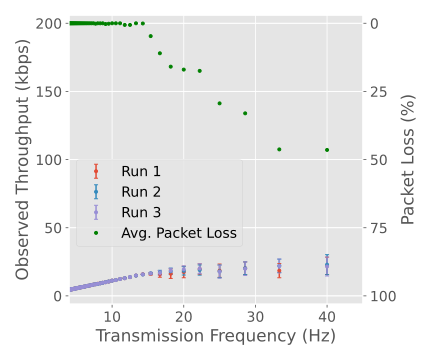
\includegraphics[width=0.75\linewidth]{images/ble-bandwidth-hci1-0cm.pdf}
    \caption[\acs{BLE} connection bandwidth obtained using the ASUS USB-BT500 adapter at a distance of 0m.]
    {\acs{BLE} connection bandwidth obtained using the Raspberry Pi 4B internal \acs{BLE} adapter at a distance of $0\text{m} \pm 0.2$. The maximum bandwidth at this distance is $23.988$ kbps, achieved at 25ms time interval between packets with 46.45\% packet loss.}
    \label{fig:ble-bandwidth-hci1-0m}
\end{figure}

\begin{figure}[H]
    \centering
    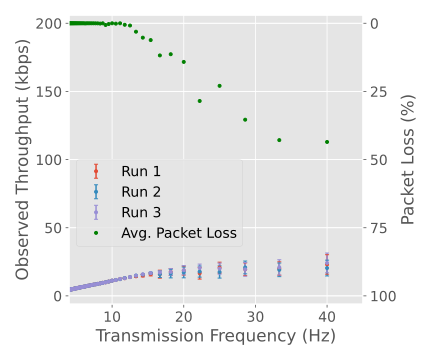
\includegraphics[width=0.75\linewidth]{images/ble-bandwidth-hci1-300cm.pdf}
    \caption[\acs{BLE} connection bandwidth obtained using the ASUS USB-BT500 adapter at a distance of 3m.]    {\acs{BLE} connection bandwidth obtained using the Raspberry Pi 4B internal \acs{BLE} adapter at a distance of $3\text{m} \pm 0.2$. The maximum bandwidth at this distance is $26.425$ kbps, achieved at 25ms time interval between packets with 41.01\% packet loss.}
    \label{fig:ble-bandwidth-hci1-3m}
\end{figure}

\begin{figure}[H]
    \centering
    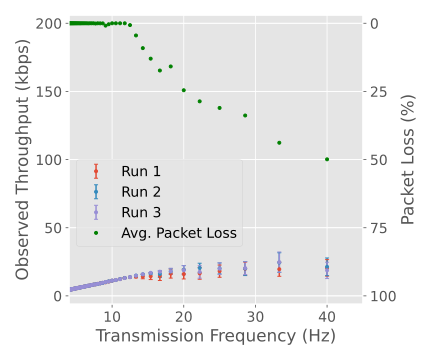
\includegraphics[width=0.75\linewidth]{images/ble-bandwidth-hci1-600cm.pdf}
    \caption[\acs{BLE} connection bandwidth obtained using the ASUS USB-BT500 adapter at a distance of 6m.]{\acs{BLE} connection bandwidth obtained using the Raspberry Pi 4B internal \acs{BLE} adapter at a distance of $6\text{m} \pm 0.2$. The maximum bandwidth at this distance is $27.188$ kbps, achieved at 30ms time interval between packets with 27.17\% packet loss.}
    \label{fig:ble-bandwidth-hci1-6m}
\end{figure}

\begin{figure}[H]
    \centering
    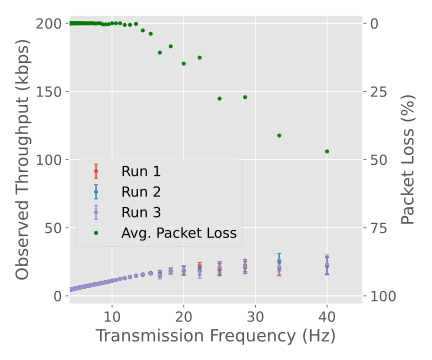
\includegraphics[width=0.75\linewidth]{images/ble-bandwidth-hci1-900cm.pdf}
    \caption[\acs{BLE} connection bandwidth obtained using the ASUS USB-BT500 adapter at a distance of 9m.]{\acs{BLE} connection bandwidth obtained using the Raspberry Pi 4B internal \acs{BLE} adapter at a distance of $9\text{m} \pm 0.2$. The maximum bandwidth at this distance is $26.556$ kbps, achieved at 30ms time interval between packets with 28.87\% packet loss.}
    \label{fig:ble-bandwidth-hci1-9m}
\end{figure}

\begin{figure}[H]
    \centering
    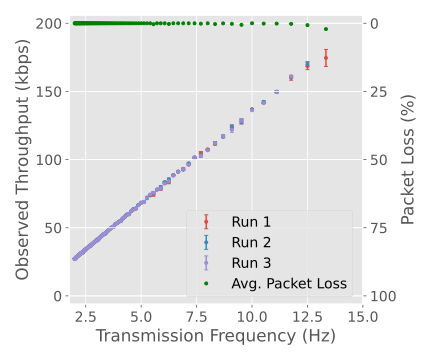
\includegraphics[width=0.75\linewidth]{images/ble-bandwidth-hci0-0cm.pdf}
    \caption[\acs{BLE} connection bandwidth obtained using the ASUS USB-BT500 adapter at a distance of 0m.]{\acs{BLE} connection bandwidth obtained using the ASUS USB-BT500 adapter at a distance of $0\text{m} \pm 0.2$. The maximum bandwidth at this distance is $178.304$ kbps, achieved at 75ms time interval between packets with 2.13\% packet loss.}
    \label{fig:ble-bandwidth-hci0-0m}
\end{figure}

\begin{figure}[H]
    \centering
    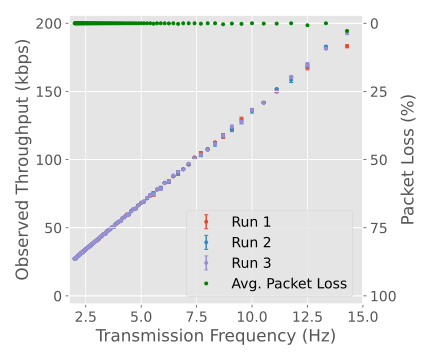
\includegraphics[width=0.75\linewidth]{images/ble-bandwidth-hci0-300cm.pdf}
    \caption[\acs{BLE} connection bandwidth obtained using the ASUS USB-BT500 adapter at a distance of 3m.]{\acs{BLE} connection bandwidth obtained using the ASUS USB-BT500 adapter at a distance of $3\text{m} \pm 0.2$. The maximum bandwidth at this distance is $194.708$ kbps, achieved at 75ms time interval between packets with 0.25\% packet loss.}
    \label{fig:ble-bandwidth-hci0-3m}
\end{figure}

\begin{figure}[H]
    \centering
    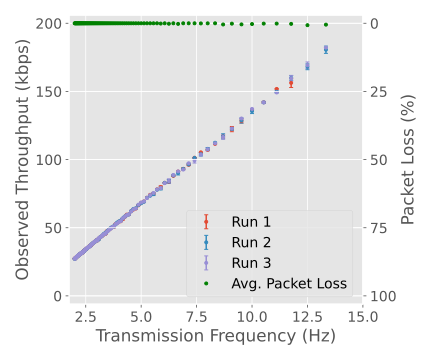
\includegraphics[width=0.75\linewidth]{images/ble-bandwidth-hci0-600cm.pdf}
    \caption[\acs{BLE} connection bandwidth obtained using the ASUS USB-BT500 adapter at a distance of 6m.]{\acs{BLE} connection bandwidth obtained using the ASUS USB-BT500 adapter at a distance of $6\text{m} \pm 0.2$. The maximum bandwidth at this distance is $182.186$ kbps, achieved at 75ms time interval between packets with 0\% packet loss.}
    \label{fig:ble-bandwidth-hci0-6m}
\end{figure}

\begin{figure}[H]
    \centering
    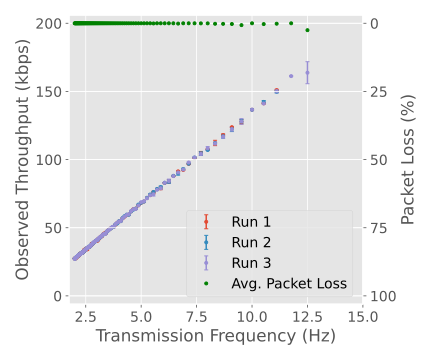
\includegraphics[width=0.75\linewidth]{images/ble-bandwidth-hci0-900cm.pdf}
    \caption[\acs{BLE} connection bandwidth obtained using the ASUS USB-BT500 adapter at a distance of 9m.]{\acs{BLE} connection bandwidth obtained using the ASUS USB-BT500 adapter at a distance of $9\text{m} \pm 0.2$. The maximum bandwidth at this distance is $166.484$ kbps, achieved at 80ms time interval between packets with 2.53\% packet loss.}
    \label{fig:ble-bandwidth-hci0-9m}
\end{figure}

As expected from the previous tests, ASUS USB-BT500 shows a much better throughput since it can transmit more data in the \acs{LL} data packets. 

\paragraph{} Additionally we observe some packet loss on the communication as time interval between packets reaches closer to the ``breaking point'' where the connection suddenly crashes, which is also expected. However, the internal \acs{BLE} adapter shows a much more noticable packet loss (particularly when the time interval between packets is higher than 100ms). Despite the heavy packet loss, we observe that the maximum observed bandwidth (accounting for the packet loss) is always achieved at the minimum time interval between packets.

\subsection{Decision on \acs{BLE} adapter}

From the previous tests, we see that the Raspberry Pi 4B's internal \acs{BLE} adapter lacks the support for \acs{DLE} feature, which reduces greatly the communication throughput. Additionally, in order to achieve this maximum throughput on Raspberry Pi 4B, we need to deal with extremely high packet loss (over 40\%!), meaning we need to either accept the packet loss, which is not feasible, or reduce the \acs{BLE} throughput to minimize the packet loss. The ASUS USB-BT500 on the other hand has a throughput 10 times bigger than the internal adapter, with very low packet loss (which can also be mitigated by reducing slightly the throughput).

\paragraph{} Due to all of the aforementioned reasons, we have decided to move forward with the ASUS USB-BT500 adapter for the development of \acs{BLE} data acquisition in the scope of the \acs{WoW} project.

\section{Summary}
In this chapter, we conducted an compreensive performance study of the different \acs{SBC}s considered for the \textit{SmartBox} development, as well as extensive analysis of the \acs{BLE} data communication.

\paragraph{} In the next chapter, we present the development of the next component in the proposed \acs{IoT} architecture -- the \textit{Smart Gateway}.